\section{Sheet Sage}
\label{sec:sheetsage}

\begin{figure*}
    \centering
    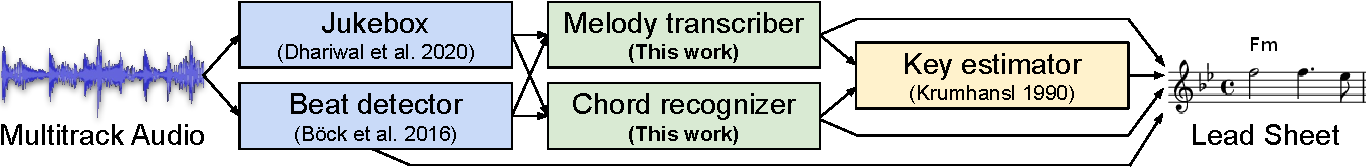
\includegraphics[width=\linewidth]{figs/sheet_sage.pdf}
    \caption{
    % TODO: Clean this up. YouTube as input
    Inference procedure for Sheet Sage, our proposed system which transcribes any Western music audio into lead sheets (scores which depict melody as notes and harmony as chord names). The blue, green, and yellow boxes respectively take audio, features, and symbolic music data as input. Green boxes are modules that we built as part of this work---both are Transformers~\cite{vaswani2017attention} trained on their respective tasks using audio features from Jukebox~\cite{dhariwal2020jukebox} and data from \hooktheory~\cite{hooktheory}.}
    \label{fig:sheet_sage}
\end{figure*}

\todo{Copied from intro. Need to integrate}
\john{Again, detail} Finally, enabled by our state-of-the-art melody transcription approach, we present \emph{\sheetsage}, a system capable of automatically transcribing Western music audio into \emph{lead sheets}. 
A lead sheet is a human-readable musical score depicting a song's melody as notes on a staff and its harmony as chord names. 
The combination of melody and harmony represents the essence of a piece of Western music, and as such, lead sheets are commonly used by experts to easily perform recognizable renditions of existing pieces. 
As part of \sheetsage, we additionally train a Transformer-based chord recognition model on \hooktheory{} data using input features from Jukebox. 
To produce lead sheets, we pair this chord recognition model with our best melody transcription model, beat detections from \madmom~\cite{bock2016madmom,bock2016joint}, key estimations from Melisma~\cite{krumhansl1990cognitive,temperley1999key,sleator2001melisma}, and engraving with LilyPond~\cite{nienhuys2003lilypond}~(\Cref{fig:sheet_sage}). 
By automatically transcribing music audio into lead sheets, our work helps reduce the gap between human perception and machine understanding of Western music.

Here we describe \sheetsage, a bonus application of our melody transcription efforts which can automatically convert music audio into lead sheets (see~\cref{sound_examples} for a demo). 
In the Western music canon, a musical composition can often be characterized by its melody and harmony. 
When engraved as a lead sheet---a musical score containing the melody as notes on a staff and the harmony as chord names---melody and harmony can be readily interpreted by musicians, enabling recognizable performances of existing pieces. 
Hence, for some music, a lead sheet represents the essence of its underlying composition.
Existing services like Chordify~\cite{de2014chordify} can already detect a subset of the information needed to produce lead sheets (specifically, chords, beats, and keys) in broad music audio. 
%chords, beats, and keys in broad music audio and output the results in musician-friendly formats like guitar tablature. 
However, despite past research efforts~\cite{ryynanen2008automatic,weil2009automatic}, no user-facing service yet exists which can convert broad music audio into lead sheets, presumably due to the poor performance of existing melody transcription systems.

To build \sheetsage, we also train a \jukebox-based chord recognition model on the \hooktheory{} data, using precisely the same methodology that we use for melody transcription (we simply replace the target vocabulary of onset pitches with one containing chord labels). 
%We use an extended chord vocabulary consisting of $96$ chord labels (major, minor, 7, maj7, m7, sus, dim, aug for each of the 12 pitch classes).
Passing audio through our \jukebox{}-based melody transcription and chord recognition models results in a score like format containing raw note names and chord labels per sixteenth note. 
Engraving this information as a lead sheet requires additional information: the key signature and the time signature. 
We estimate the former using the Krumhansl-Schmuckler algorithm~\cite{krumhansl1990cognitive,temperley1999key}, which takes the symbolic melody and chord information as input. 
For the latter, we use \madmom~\cite{bock2016madmom,bock2016joint} to estimate beats and downbeats from the audio, which implicitly gives us the time signature.
Finally, we engrave a lead sheet using Lilypond~\cite{nienhuys2003lilypond}. 
See~\Cref{fig:sheet_sage} for a schematic of our system.

On pop music, \sheetsage{} often produces near-perfect lead sheets, especially for the chorus and verse segments which have more prominent melodies. 
It can even successfully track the melody as it changes across instruments. 
Performance is fairly robust across broad genres and instruments which are less represented in the training data---one user reported particularly strong success on Bollywood music. 
However, the system occasionally struggles, especially with certain vocal styles, multiple monophonic harmonies, or poor intonation. 
Additionally, because the system takes detected beats and downbeats as an first-stage input, results can suffer when these estimates are poor. 
\sheetsage{} is also limited by its current system design: it can only handle $3$/$4$ or $4$/$4$ time signatures and cannot handle key or time signature changes. 
Overcoming these system limitations would involve either (1)~research into downbeat detection and key estimation which supports time / key signature changes, or (2)~user intervention to provide the correct information.